
\begin{frame}{kpi}
  \begin{center}
    \movie[autostart,loop]{
    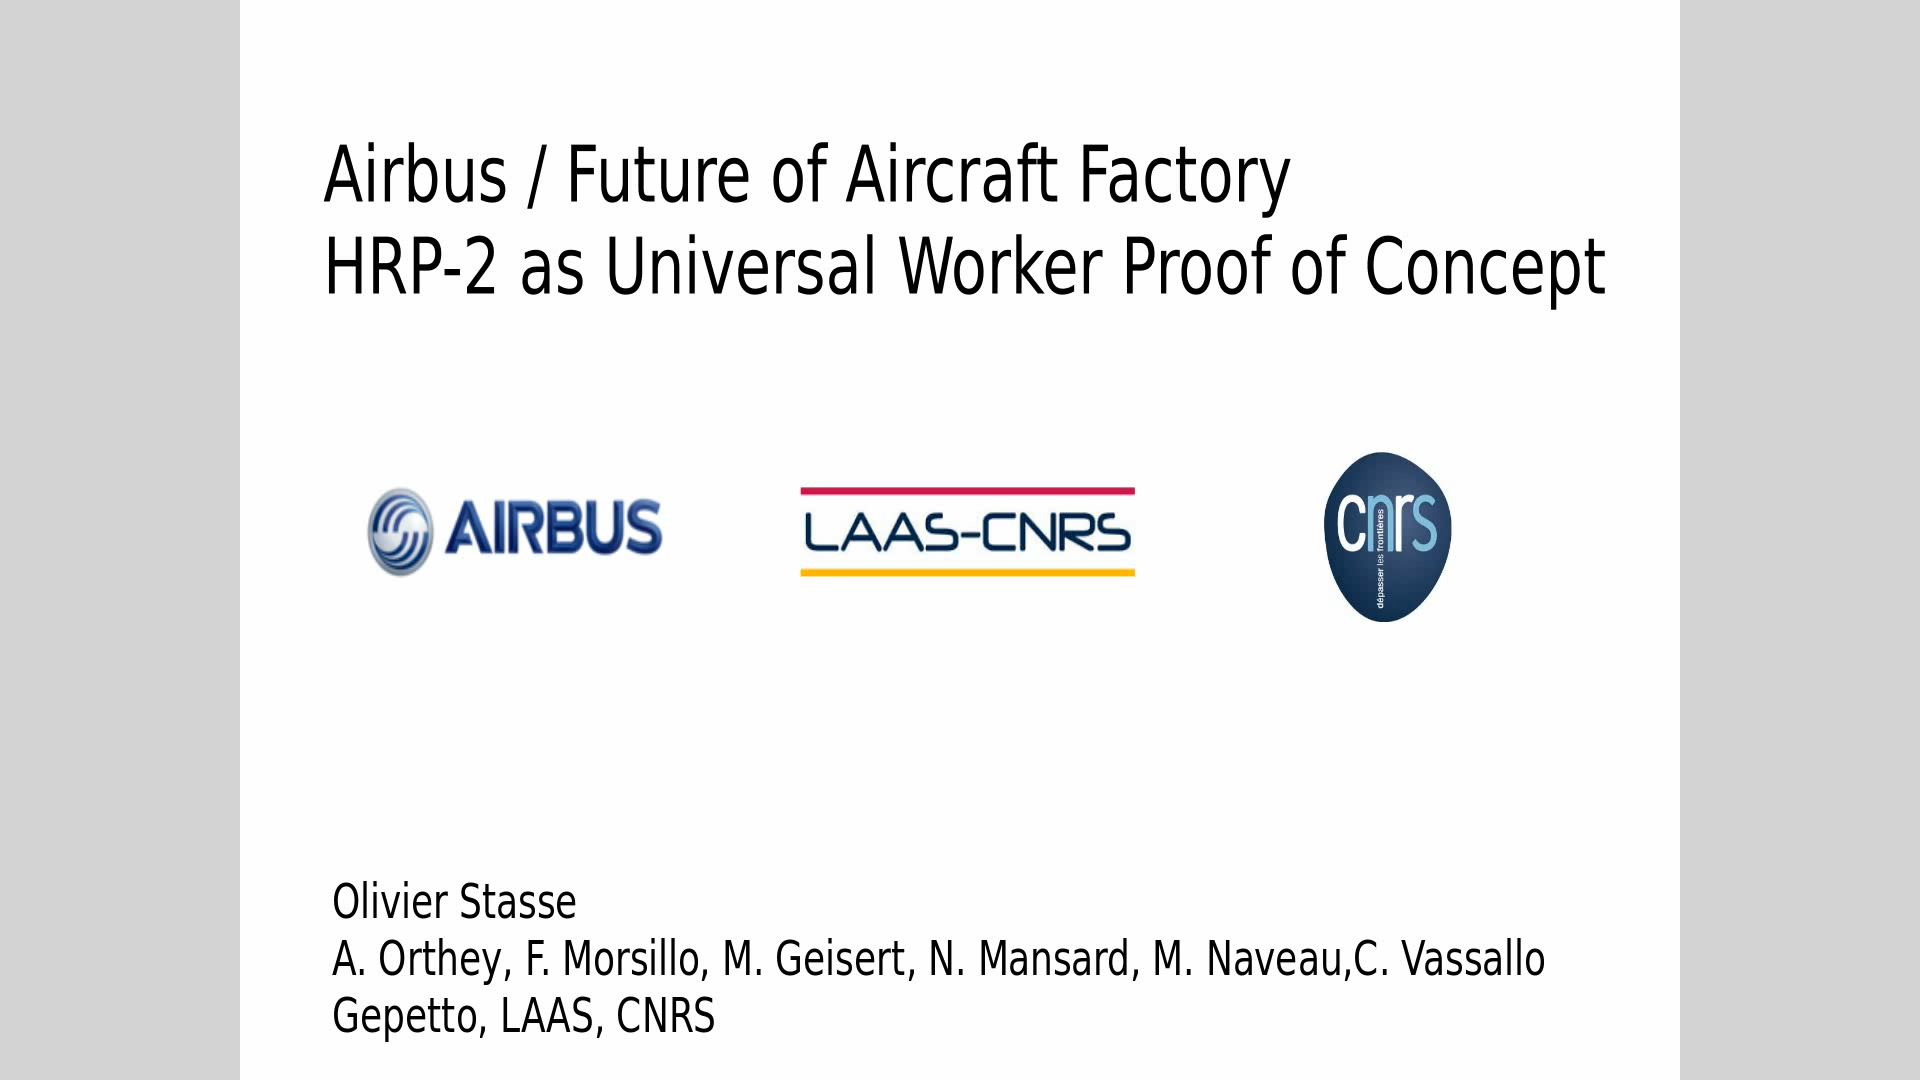
\includegraphics[width=0.4\linewidth, keepaspectratio]
      {poc_airbus/PocAirbus2013_12_Short.png}    
    }  
    {./videos/Koroibot-HRP2-GoingUp15cmLateralView.avi}
    \movie[autostart,loop]{
    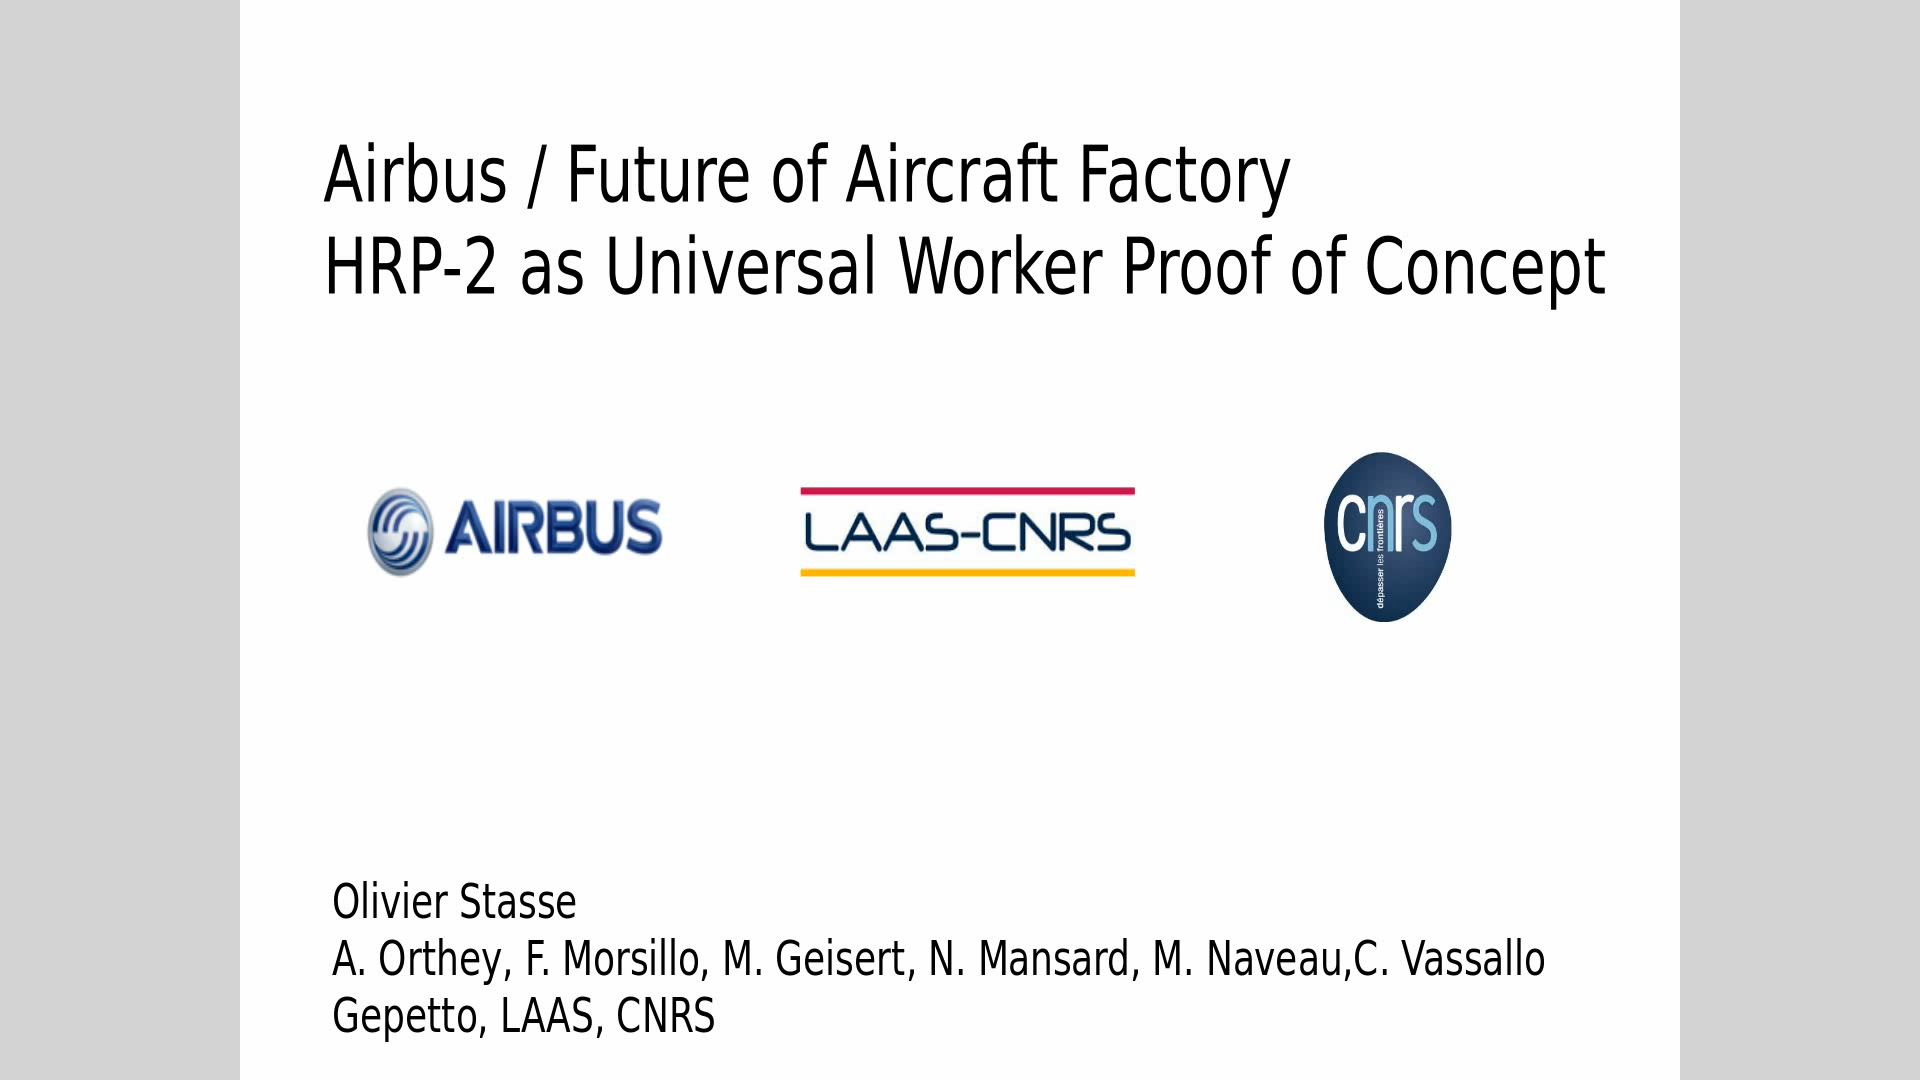
\includegraphics[width=0.4\linewidth, keepaspectratio]
      {poc_airbus/PocAirbus2013_12_Short.png}    
    }
    {./videos/Koroibot-HRP2-GoingUp10cmLateralViewv2.avi}
    \movie[autostart,loop]{
    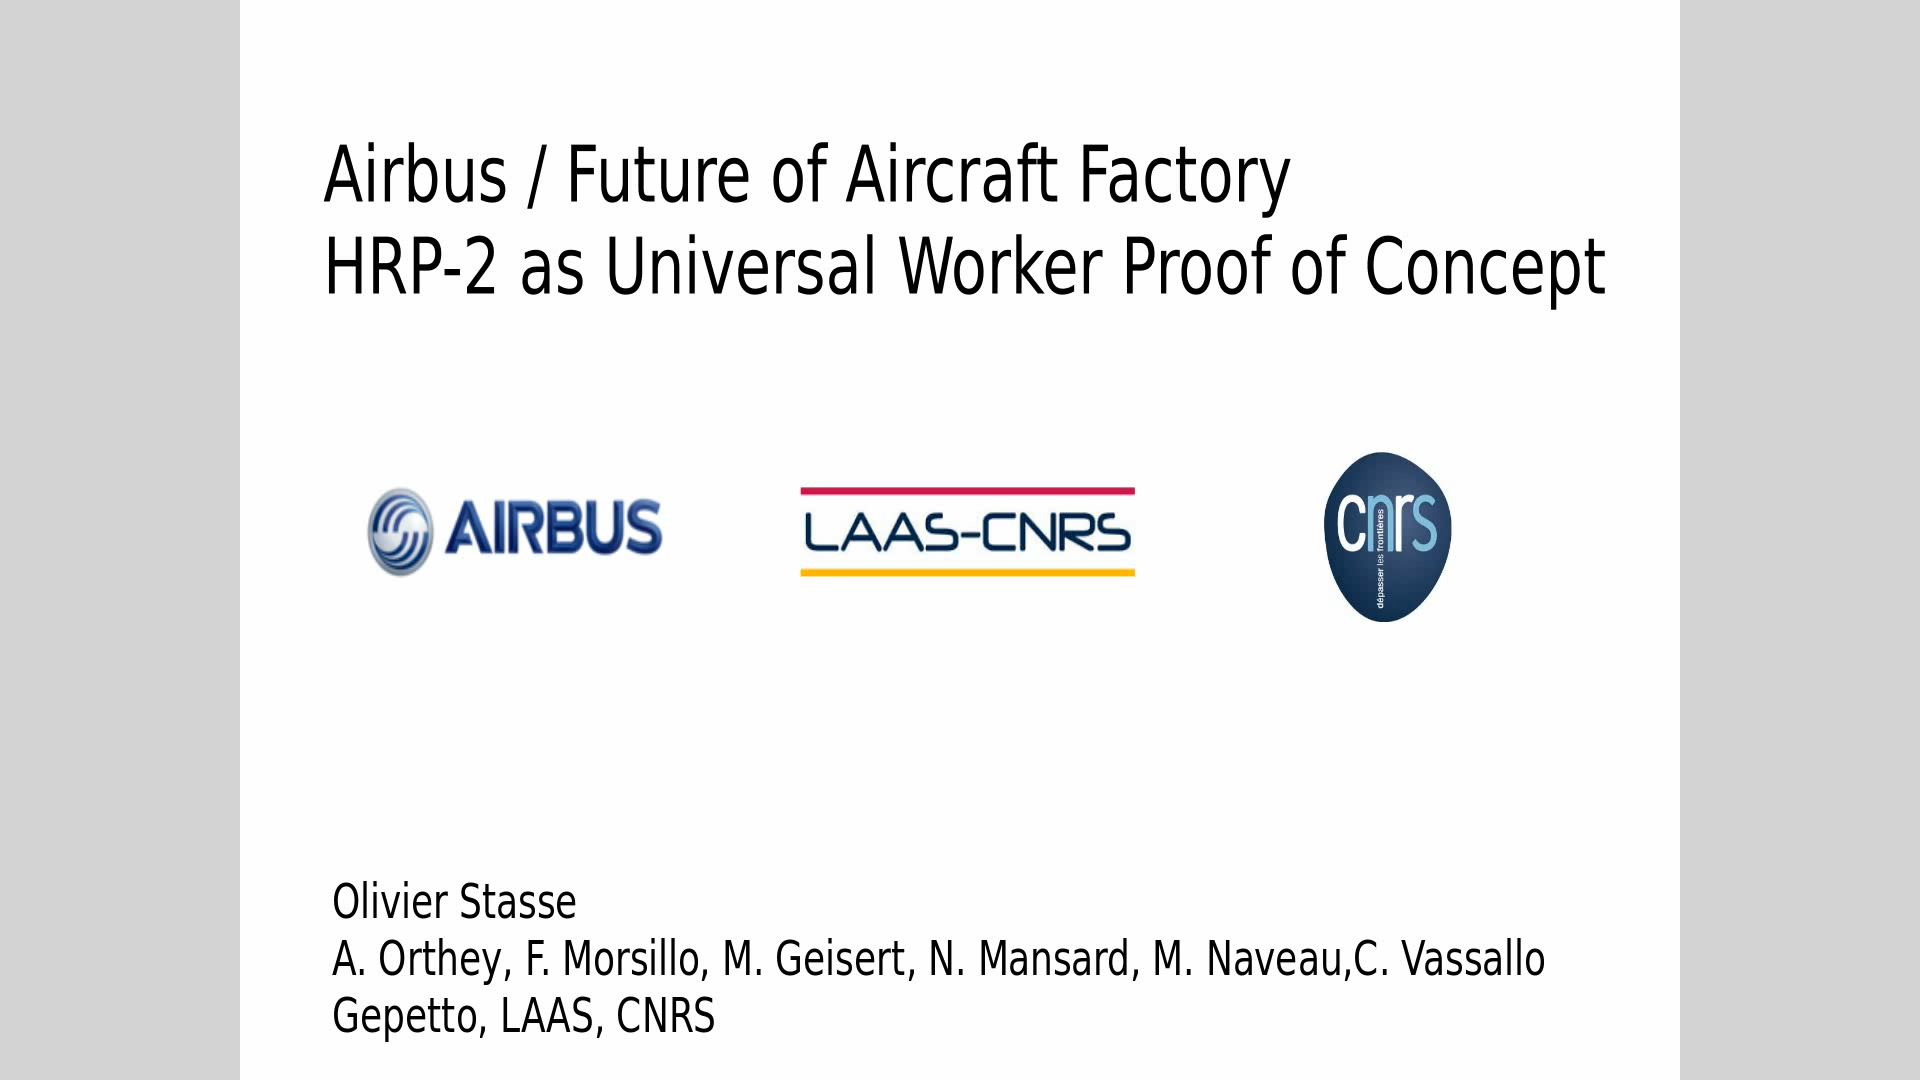
\includegraphics[width=0.4\linewidth, keepaspectratio]
      {poc_airbus/PocAirbus2013_12_Short.png}    
    }  
    {./videos/Koroibot-HRP2-SteppingStonesLateralView.avi}
    \movie[autostart,loop]{
    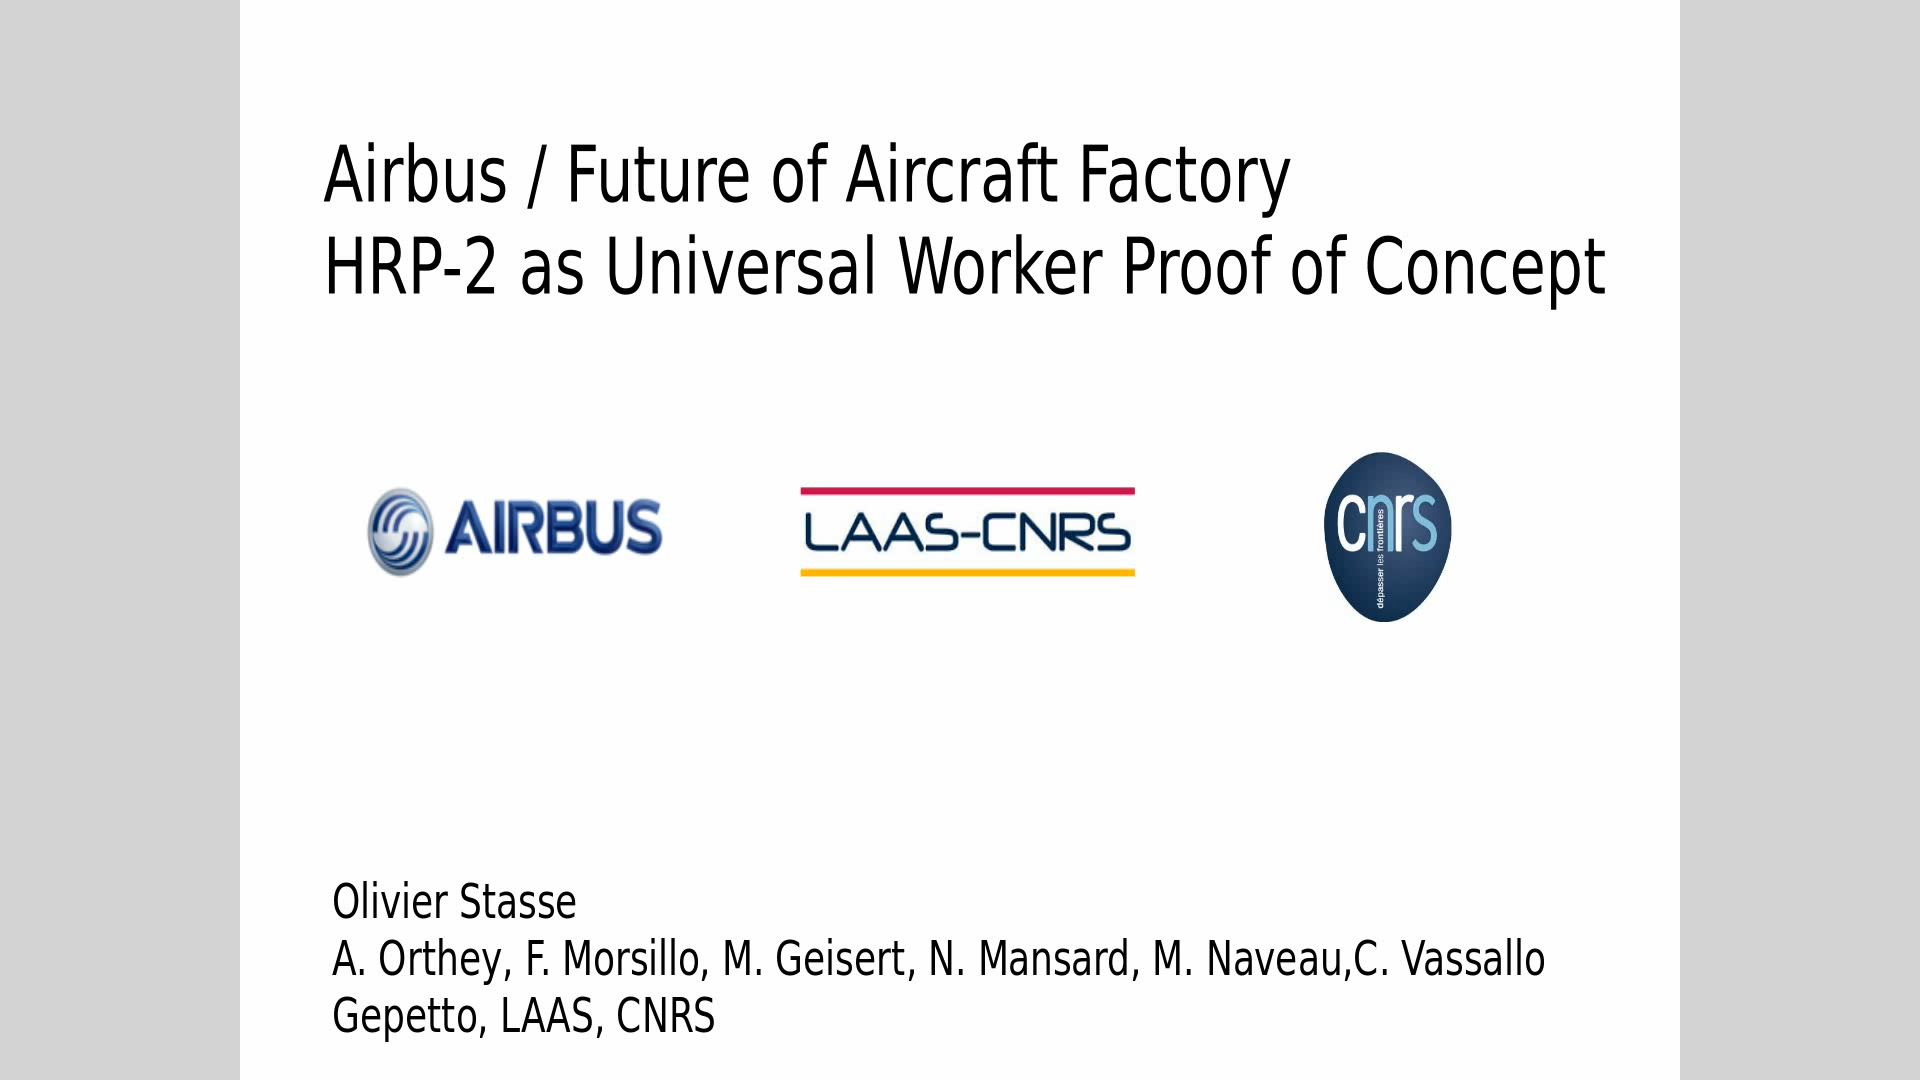
\includegraphics[width=0.4\linewidth, keepaspectratio]
      {poc_airbus/PocAirbus2013_12_Short.png}    
    }  
    {./videos/Koroibot-HRP2-WalkingOnBeam_v3.mp4}
  \end{center}
\end{frame}

\begin{frame}{Different Problematics}

\begin{itemize}
  \item flat ground walking
  \begin{itemize}
    \item small step length ($5cm/step$)
    \item need planner for advanced application (like obstacle avoidance)
    \item important drift during rotation ($90deg$ in two laps of an ellipse)
  \end{itemize}
  
  \item stair walking
  \begin{itemize}
    \item important energy consumption ($5$ times more than flat ground walking)
  \end{itemize}
  
  \item beam walking
  \begin{itemize}
    \item no sensor feedback
  \end{itemize}
\end{itemize}
\begin{tikzpicture}[remember picture, overlay]
  \draw [draw=red,sloped,line width=15pt,->] (0.5,0.5) -- node {\color{white}{\textbf{Reactivity Functionnality}}} (11.0,5.0);
\end{tikzpicture}
\end{frame}